% ****** Start of file apssamp.tex ******
%
%   This file is part of the APS files in the REVTeX 4.1 distribution.
%   Version 4.1r of REVTeX, August 2010
%
%   Copyright (c) 2009, 2010 The American Physical Society.
%
%   See the REVTeX 4 README file for restrictions and more information.
%
% TeX'ing this file requires that you have AMS-LaTeX 2.0 installed
% as well as the rest of the prerequisites for REVTeX 4.1
%
% See the REVTeX 4 README file
% It also requires running BibTeX. The commands are as follows:
%
%  1)  latex apssamp.tex
%  2)  bibtex apssamp
%  3)  latex apssamp.tex
%  4)  latex apssamp.tex
%
\documentclass[%
 reprint,
 amsmath,amssymb,
 aps,prl,
 showpacs,
 linenumbers
]{revtex4-1}

\usepackage{graphicx}% Include figure files
\usepackage{dcolumn}% Align table columns on decimal point
\usepackage{bm}% bold math


\begin{document}

\preprint{APS/123-QED}


\title{Extracellular processing of molecular gradients by eukaryotic cells can improve gradient detection accuracy}

\author{Igor Segota}
 \altaffiliation[Present address: ]{Department of Physics, University of California San Diego}
%Lines break automatically or can be forced with \\
 \email{is246@cornell.edu}
\author{Carl Franck}%
 %\email{Second.Author@institution.edu}
\affiliation{Laboratory of Atomic and Solid State Physics, Cornell University, Ithaca 14853, USA}

\date{\today}

\begin{abstract}

Eukaryotic cells sense molecular gradients by measuring spatial concentration differences through the difference in the number of occupied receptors to which molecules can bind. They also secrete enzymes that degrade these molecules, and it is presently not well understood how this affects the local gradient perceived by cells. Numerical and analytical results show that these enzymes can substantially increase signal-to-noise ratio of the receptor difference and allow cells to respond to a much broader range of molecular concentrations and gradients. 

\end{abstract}

\pacs{87.17.Jj, 82.39.Fk, 87.10.Ed, 87.10.Kn} % PACS, the Physics and Astronomy
\maketitle

%
%
% Introduction
%
%
Eukaryotic cells sense and follow molecular concentration gradients
in a process called chemotaxis. This process is essential for numerous biological functions
such as proliferation, organ formation, wiring of the nervous system,
wound healing and cancer \cite{review1,cancer-rev,zigchemotaxis}.
In contrast to bacteria \cite{bacteriaChemo}, eukaryotic cells are
large enough ($\gtrsim10\,\mu\mathrm{m}$) to be able
to directly measure concentration differences across their bodies
\cite{bergpurcell}. This is achieved by taking
snapshots of the non-uniform occupancy of their cell surface receptors
to which diffusing molecules can bind.

The physical limits of chemotactic sensitivity in eukaryotic cells
have been extensively studied both theoretically and experimentally,
often by calculating theoretical limits and then comparing the accuracy
of the experimental chemotaxis response to these limits \cite{bergpurcell,wing1,wing2,
rappelherbie1,rappelherbie2,rappelherbie3,fuller-1,shib,song,eberhard1,eberhard2,me}.
However, since many cells secrete enzymes that can inactivate chemotactic signals, the local gradient near the cell surface may differ from the gradient away from the cell.

% Figure 1.
\begin{figure}[t]
	\centering
	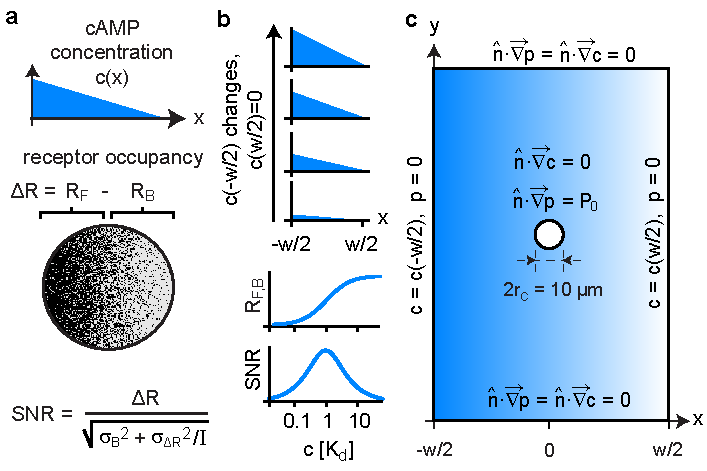
\includegraphics[scale=0.7]{../figures/fig1}
	\caption{\linespread{1.0}\selectfont{}Signal-to-noise ratio (SNR) and model geometry. 
	\textbf{a}. SNR is defined as the receptor difference between the front half and back half of the cell (signal) divided by the noise consisting of receptor shot noise $\sigma_{\Delta R}$ sampled $I$ times and non-receptor noise $\sigma_B$.
	\textbf{b}. When the relative gradient $|\vec{\nabla}c|/c = \mathrm{const.}$, the optimal average concentration that maximizes SNR is $c=K_d$, since the receptor occupancy difference $\Delta R$ has maximum when $c=K_d$ and $\mathrm{SNR} \propto \sqrt{\Delta R}$.
	\textbf{c}. Geometry and boundary conditions for 3D numerical simulations; $c$ = cAMP, $p$ = PDE concentration (not to scale). Constant relative gradient can be set away from the cell (in the bulk), by changing the cAMP concentration on the left boundary $c(-w/2)$, while keeping $c(w/2) = 0$. $w = 1\,\mathrm{mm}$.
	}
	\label{fig:geom}
\end{figure}
For example, \emph{Dictyostelium discoideum} cells secrete phosphodiesterases (PDE) \cite{PDE} that inactivate cyclic adenosine monophosphate (cAMP) signals \cite{kessinBook}, \emph{Saccharomyces cerevisiae} cells secrete Bar1 protease that degrades $\alpha$-factor pheromone \cite{yeast1,yeast2,yeast3} and neutrophils can inactivate chemotactic formylmethionyl peptides \cite{zigchemotaxis}.
More recently, it has been suggested that the PDE inactivation can steepen cAMP gradients in \emph{D. discoideum} (\cite{kessinBook}, p.125) or improve the gradient direction alignment with the direction of the nearest mating partner in \emph{S. cerevisiae} \cite{yeast1,yeast2,yeast3}.

In \emph{D. discoideum}, PDE exists in membrane bound and a secreted extracellular form \cite{PDE,pde2,pde3,pde-purification}, both encoded by the same gene \emph{pdsA}. Nanjundiah and Malchow \cite{mechanism1} argued, using dimensional analysis, that the extracellular PDE has no observed effect. More recently, Palsson et al. \cite{palsson0,palsson1,palsson2} showed that within the particular parameter range of their model, PDE becomes important for wave propagation at low cell densities. Experimentally, \emph{D. discoideum} \emph{pdsA-} strain (deleted PDE gene) has been shown to fail to aggregate \cite{pde-knockouts1,pde-knockouts2} and to respond to a reduced range of cAMP concentrations compared to wild-type \cite{pdsA1}. Despite these efforts, it remains poorly understood how exactly extracellular PDE affects the local cAMP gradient perceived by cells.

We address this question by calculating cAMP concentration around the cell using 3D reaction-diffusion models of cAMP-PDE interaction in the extracellular space, for a typical microfluidic geometry \cite{me,wu} and in space where a cell is detecting cAMP emitted by a point source. 
We use these results to calculate the gradient detection signal-to-noise ratio (SNR) of the receptor response following Rappel and Levine \cite{rappelherbie2} and van Haastert and Postma \cite{SNRvh} and predict how the chemotaxis index is affected by extracellular PDE.

We can gain some intuition about SNR by considering a linearly increasing cAMP concentration $c(x)$ in 1D.  
Assuming the steady state of cAMP to cAMP-receptor binding, each receptor at coordinate $x$ can be thought of as a Bernoulli trial with the probability of being occupied $p(x) = c(x)/[c(x) + K_d]$ and unoccupied with probability $1-p(x)$, where $K_{d}$ is the cAMP to cAMP-receptor binding dissociation constant (SI, Section 1).
Since the receptor distribution on the cell surface is uniform \cite{uniform_receptor_distribution} and cAMP concentration $c(x) = c_0 -|\vec{\nabla} c|x$, we can consider having half receptors on each cell half at $x = \mp r_c/2$ ($r_c$ is cell radius, cell is centered at $x=0$). The distribution of the number of occupied receptors on each half of the cell follows a Binomial distribution with the average and variance:
\begin{equation}
	R_{F,B} = \frac{N}{2} \frac{c_{F,B}}{c_{F,B} + K_d},\quad
	\sigma_{R_{F,B}}^{2}= \frac{N}{2} \frac{c_{F,B} K_d}{(c_{F,B} + K_d)^2}
	\label{eq:RFB}
\end{equation}
where $c_{F,B} = c(\mp r_c/2)$ and $N$ is the total number of receptors per cell; here $K_d=30\,\mathrm{nM}$, $N=70,000$ \cite{RtKdcAR1}. 
%Since $N\gg1$, Binomial distribution can be approximated with Normal distribution so $R_F$, $R_B$ and $\Delta R=R_{F}-R_{B}$ are all Normally distributed \cite{normalDifference}. 
SNR is defined as \cite{SNRvh, rappelherbie2} (Fig.\ref{fig:geom}a):
\begin{equation}
	\mathrm{SNR}=\frac{\Delta R}{\sqrt{\sigma_B^2+\sigma_{\Delta R}^2/I}}, \Delta R = R_F-R_B
	\label{eq:SNRdef}
\end{equation}
where $\Delta R$ and $\sigma_{\Delta R}^2 = \sigma_{R_F}^2 + \sigma_{R_B}^2$ are the average (``signal'') and variance (square of the ``noise'') of the difference of occupied receptors at the front and back half of the cell, $\sigma_B$ the non-receptor noise and $I$ is the the number of statistically independent measurements of the occupied receptors \cite{SNRvh}.

For shallow gradients, the concentration difference between the cell front and back is small ($r_c |\vec{\nabla} c| \ll K_d$) so the average and variance of the receptor difference are (SI, Section 2):
\begin{equation}
	\Delta R \approx \frac{N}{2}\frac{K_d r_c |\vec{\nabla} c|}{\left(c_0 + K_d\right)^2},\quad 
	\sigma_{\Delta R}^2 \approx N \frac{c_0 K_d}{\left(c_0 + K_d\right)^2}
	\label{eq:signal_noise_def}
\end{equation}
For fixed relative gradients $|\vec{\nabla} c|/c_0 = \mathrm{const.}$: (i)  the receptor occupancy $R_{F,B}$ has the steepest increase at $c_0=K_d$, so $\Delta R \propto dR/dc$ is maximal, and (ii) the receptor noise is proportional to the square root of the signal $\sigma_{\Delta R} \propto \sqrt{\Delta R}$. Then, SNR is also proportional to the square root of the signal: $\mathrm{SNR} \propto \Delta R/ \sqrt{\Delta R} = \sqrt{\Delta R}$ and also maximal at $c_0 = K_d$ (Fig.\ref{fig:geom}b). Therefore, the optimal average cAMP concentration for gradient sensing without PDE is at exactly $K_d$ when the receptor occupancies are $\approx 50\%$.

For parameter values $\sigma_{B}=73$ and $I=1.4$ the measured chemotaxis index (CI) was fit to the empirical equation $\mathrm{CI} = \mathrm{SNR}/(\mathrm{SNR} + 1)$; see SI Section 3.

%
%
%  Fixed PDE secretion flux model
%
%
\emph{Fixed PDE secretion flux model.}--- We consider a system of two interacting molecules, PDE and cAMP, following
Michaelis-Menten kinetics:
\begin{equation}
	\mathrm{PDE+cAMP}\overset{k_{1}}{\underset{k_{-1}}{\rightleftharpoons}}C_{cp}\overset{k_{2}}{\rightharpoonup}\mathrm{PDE+5'AMP}
	\label{eq:PDEcAMPint}
\end{equation}
where $k_i$ represent the reaction rates, $C_{cp}$ represents the intermediate cAMP-PDE complex and
5'AMP the product of this reaction (a deactivated signal).

% Figure 2. Fixed PDE secretion flux model results.
\begin{figure}[!th]
	\centering
	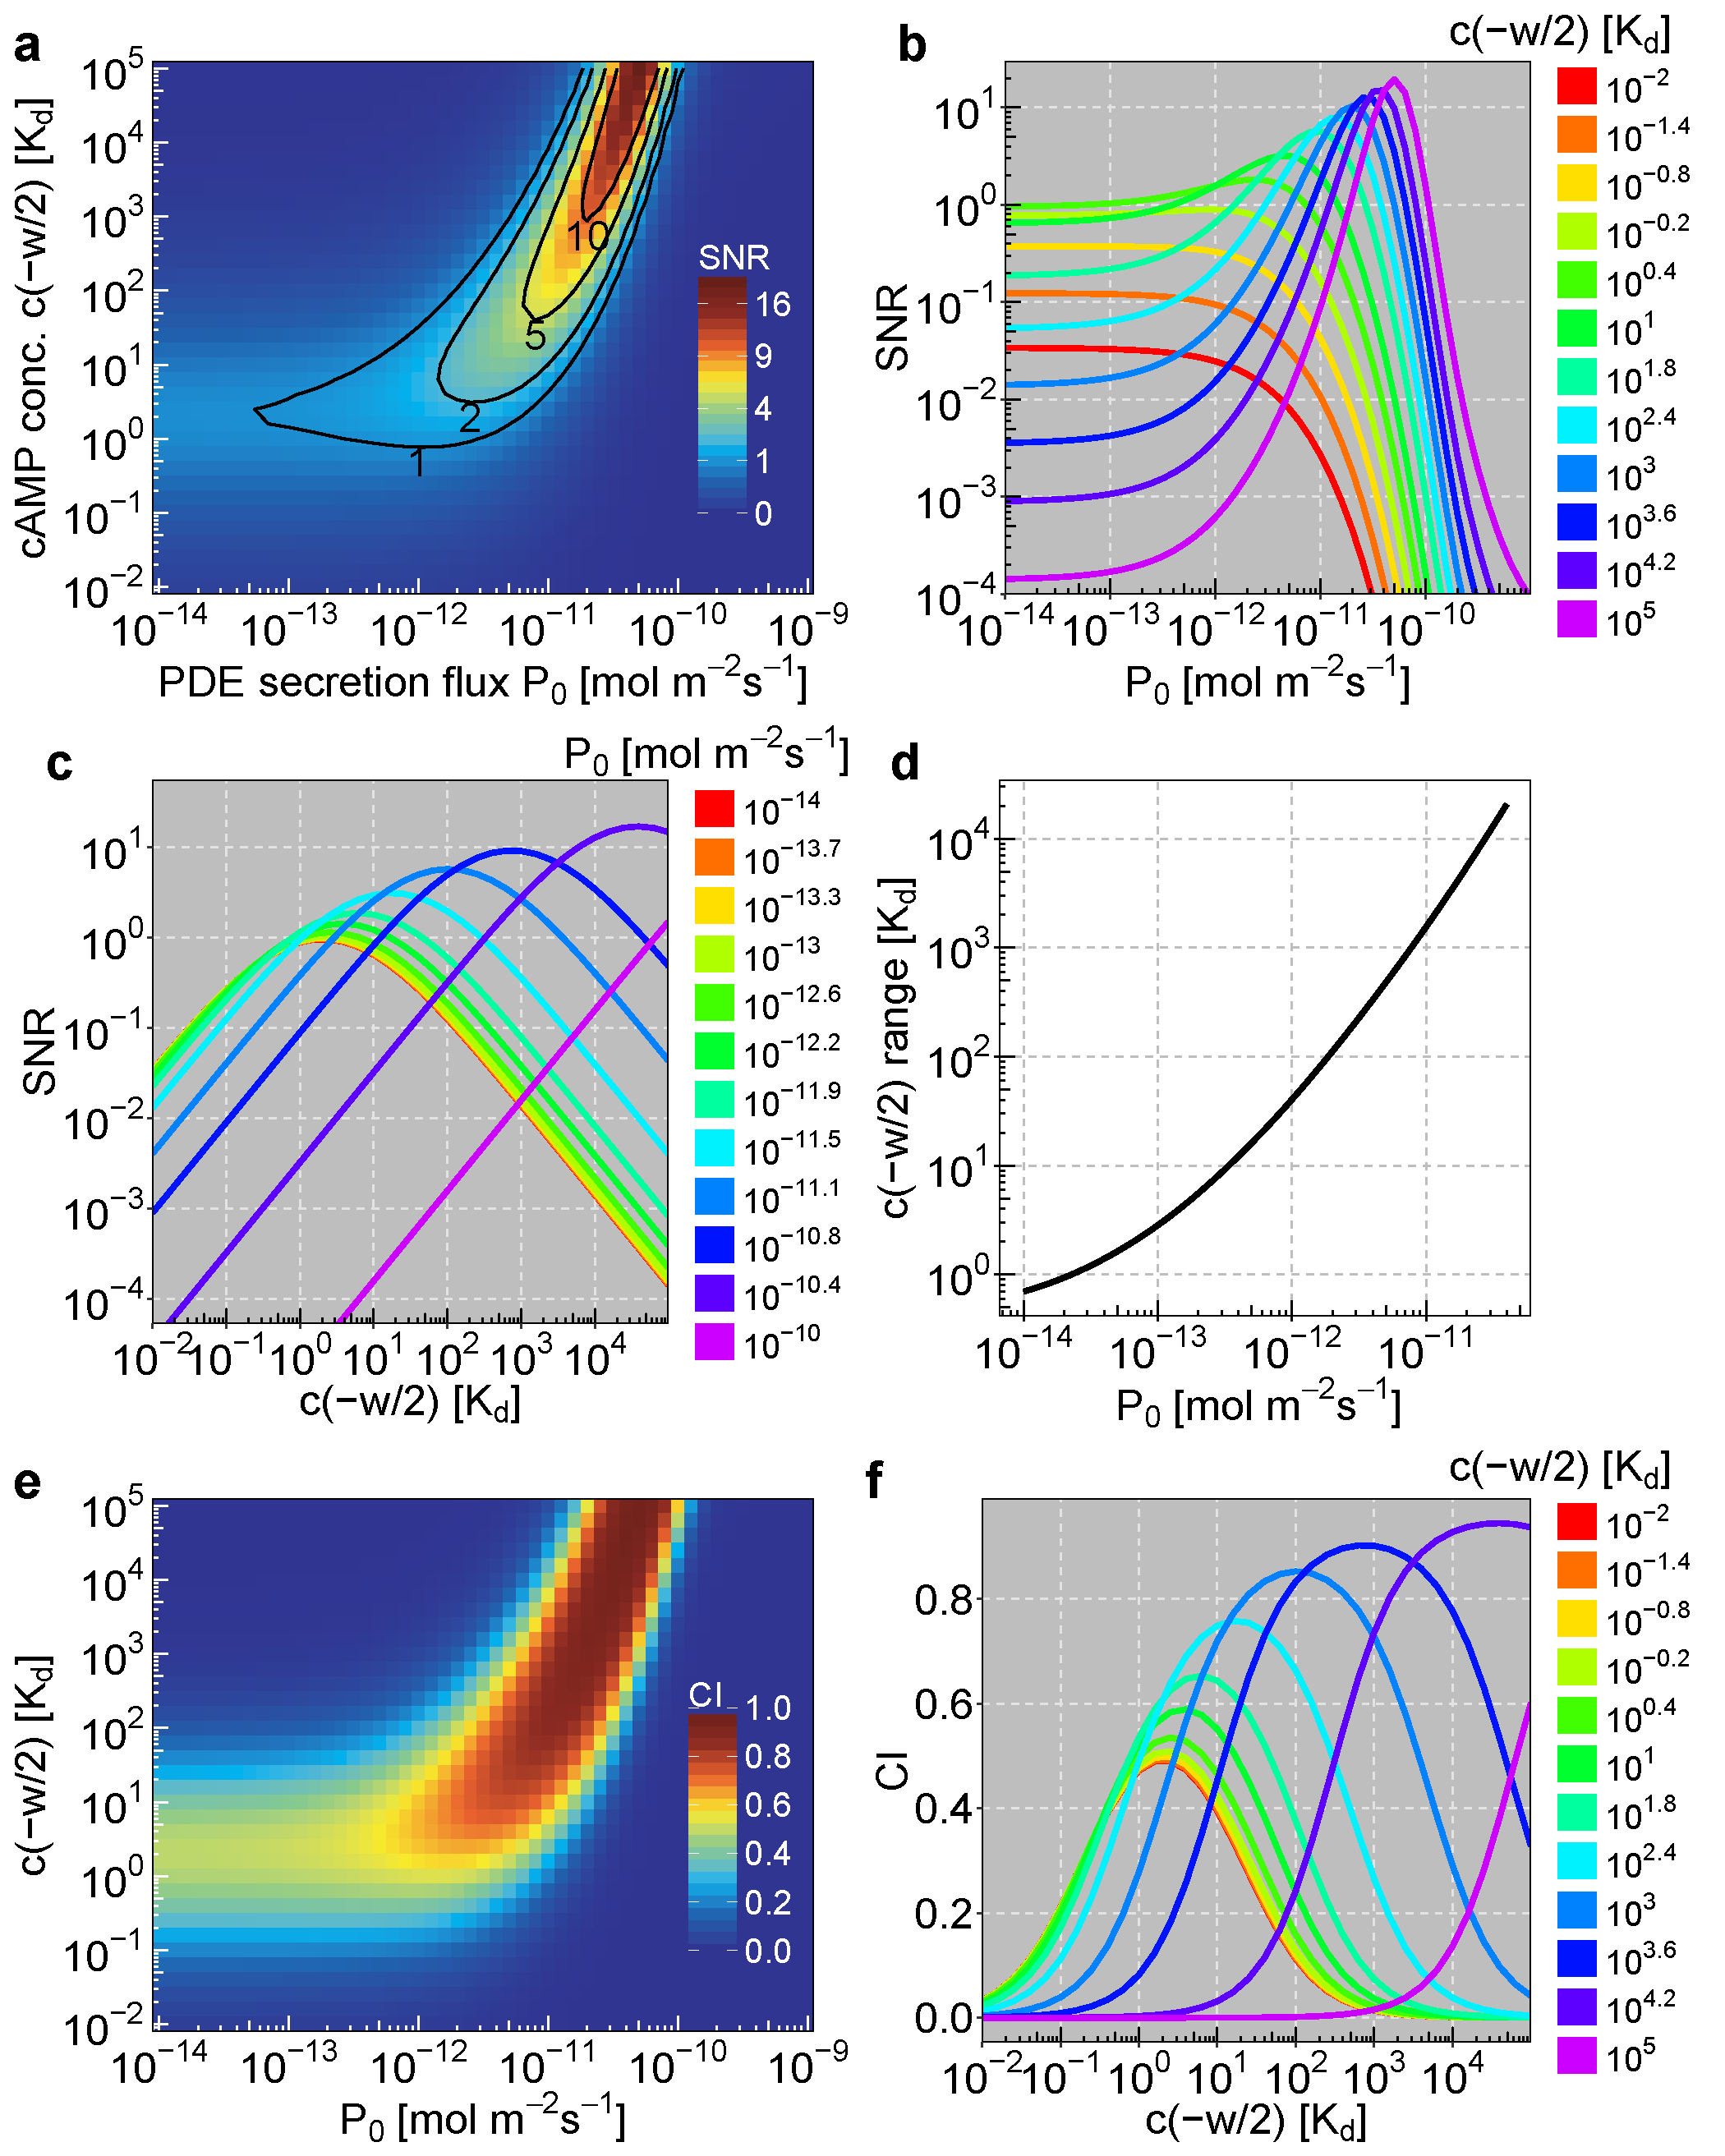
\includegraphics[scale=0.25]{../figures/fig2_pde_flux_plots}
	\caption{
		\linespread{1.0}\selectfont{}Fixed PDE secretion flux model with relative gradient on the cell body
		is $1\%$.
		\textbf{a}. SNR as a function of PDE secretion flux $P_0$ and cAMP boundary
		concentration $c(-w/2)$. SNR can be substantially improved by PDE for a range of 
		parameters $P_0$ and $c(-w/2)$.
		\textbf{b}. Horizontal slices from a. PDE can increase SNR for $c(-w/2) \gtrsim  K_d$.
		\textbf{c}. Vertical slices from a. Increasing $P_0$ shifts the optimal cAMP concentration (maximizing SNR) towards higher values but also broadens the detectable range of cAMP concentrations. The red curve for $P_0 = 10^{-14}\,\mathrm{mol\,m^{-2} s^{-1}} \approx 0$, i.e. matches SNR in Fig.\ref{fig:geom}b.
		\textbf{d}. Broadening of curves from c is quantified by calculating the range of $c(-w/2)$ for which $\mathrm{SNR} \geq 1$.
		\textbf{e}. Chemotaxis index (CI) calculated as $\mathrm{SNR}/(\mathrm{SNR}+1)$ (SI Section 3).
		\textbf{f}. Vertical slices from e. 
	}
	\label{fig:Results1}
\end{figure}

The concentrations of cAMP $c(\vec{r},t)$, PDE $p(\vec{r},t)$, cAMP-PDE complex
$C_{cp}(\vec{r},t)$ and the 5'AMP $c'(\vec{r},t)$, are obtained in the standard quasi-steady
state assumption \cite{QSSA} (intermediate complex is in steady state): $k_{1}cp=(k_{-1}+k_{2})C_{cp}$, so the two relevant steady-state equations are (SI, Section 4):
\begin{equation}
		D_c\nabla^{2}c-\frac{k_2}{K_M}pc = 0, \quad
		D_p\nabla^{2}p = 0
  \label{eq:main_sys}
\end{equation}
where $D_c$ and $D_p$ are the diffusion constants of cAMP and PDE and $K_M \equiv (k_{-1}+k_2)/k_1$. 
These equations are solved numerically using COMSOL 3.5 (Comsol Inc.) with MATLAB R2011a (The MathWorks, Inc.) for the boundary conditions mimicking typical experiments \cite{me,varnumsollStatic,fisherStatic}, (Fig.\ref{fig:geom}c and SI Section 5). 
cAMP concentration is varied on the left boundary $c(x{=}{-}w/2)$, zero on the right boundary $c(x{=}w/2) = 0$ and the normal component of cAMP flux is zero everywhere else, including the cell boundary \footnote{Zero-normal cAMP flux seems reasonable since the time scale for receptor internalization is 5 minutes [A. Serge et al. Integr. Biol., 3, 675-683, 2011] compared to the time scale of receptor dissociation of 1 second [M. Ueda et al. Science, 294, 864-867, 2001], so the binding and unbinding processes are in equilibrium.}. These boundary conditions result in constant applied relative gradient $|\vec{\nabla}c|_{\mathrm{app}}/c_{0,\mathrm{app}}$, where $|\vec{\nabla}c|_{\mathrm{app}} = [c(-w/2) - c(w/2)]/w = c(-w/2)/w$ and $c_{0,\mathrm{app}} = [c(-w/2) + c(w/2)]/2 = c(-w/2)/2$. 
For PDE concentration, $p(x{=}\pm w/2) = 0$ and its normal flux is zero everywhere except for the cell boundary where it is $P_0$.
The parameters used in simulations were: $K_M=10\,\mathrm{\mu M}$ \cite{KmcAMPPDEandPDI}, $D_{c}=444\,\mathrm{\mu m^{2}s^{-1}}$ \cite{DcAMP}, $D_{p}=70\,\mathrm{\mu m^{2}s^{-1}}$, $k_{2}=13,300\,\mathrm{s^{-1}}$(estimated; SI, Section 6), $r_c = 5\, \mathrm{\mu m}$. 

Fig.\ref{fig:Results1}a shows SNR, as a function of PDE secretion flux $P_0$ and cAMP concentration on the left boundary $c(-w/2)$, for the relative gradient $r_c|\vec{\nabla} c|_{\mathrm{app}}/c_{0,\mathrm{app}} = 2r_c/w = 1 \%$ across the cell body. 
PDE can substantially improve SNR for a range of $P_0$ and $c(-w/2)$ values and the improvement is better for large cAMP concentrations. If the midpoint concentration is $\lesssim K_d$ ($c(-w/2) \lesssim 2\, K_d$), then SNR can only be decreased by PDE (Fig.\ref{fig:Results1}b). PDE can also broaden the range of cAMP detection by increasing the $c(-w/2)$ range for which $\mathrm{SNR} \geq 1$ (Fig.\ref{fig:Results1}c,d). This behavior is also reflected in the CI (Fig.\ref{fig:Results1}e,f). The SNR improvement by PDE also occurs when either the absolute gradient $|\vec{\nabla}c|_{\mathrm{app}}$ or the midpoint concentration $c_{0,\mathrm{app}}$ are fixed (SI, Section 7).

According to Fig.\ref{fig:Results1}, the relevant $P_0$ range between $10^{-12}$ and $10^{-10}\,\mathrm{mol\, m^{-2}s^{-1}}$, falls within the rough physiological range estimated here for PDE of $10^{-11}\,\mathrm{mol\, m^{-2}s^{-1}}$ (SI Section 6.3) and by others for Bar1 of $10^{-12}\,\mathrm{mol\, m^{-2}s^{-1}}$ (which degrades $\alpha$-factor pheromone signal in yeast) \cite{yeast2}.

Next, we analyze how the increase in SNR is achieved. PDE reduces the gradient but even more the average concentration across the cell body (Fig.\ref{fig:pde_flux_signal_noise}a), so the signal $\Delta R \propto |\vec{\nabla}c|/(c_0 + K_d)^2$ is enhanced (Fig.\ref{fig:pde_flux_signal_noise}b). For $P_0 \lesssim 10^{-10}\,\mathrm{nM\,\mu m^{-1}}$, PDE can generate up to $\sim 1000$ receptors difference.
On the other had, the noise has both an upper bound of $\sqrt{\sigma_B^2 + N/(4I)} \approx 134$ at $c_0 = K_d$ (Eq.\ref{eq:signal_noise_def}) and a lower bound due to the non-receptor noise $\sigma_B = 73$ (Fig.\ref{fig:pde_flux_signal_noise}c). Both bounds follow directly from the definition, Eqs.\ref{eq:SNRdef},\ref{eq:RFB} and imply that the overall scale of the noise is largely PDE-independent. 
This results in the SNR enhancement that comes directly from the signal increase, which can be more than an order of magnitude for $c_0 \gtrsim 100\,K_d$ (Fig.\ref{fig:pde_flux_signal_noise}d).


%
%
% Fixed PDE concentration models
%
%
\emph{Fixed PDE concentration models.}--- We consider two models with spatially uniform PDE concentration $p(\vec{r},t) = p_0$. For the case with same microfluidic geometry as before but without cell boundary in the middle, the exact analytical solution of Eq.\ref{eq:main_sys} is:
\begin{equation}
	c(x) = c(-w/2) \frac{\sinh\left(\frac{w}{2L}-\frac{x}{L}\right)}
		{\sinh\left(\frac{w}{L}\right)},\quad L=\sqrt{\frac{K_M D_c}{k_2p_0}}
	\label{eq:uniform_pde_analytic_sol}
\end{equation}
where now a degradation length $L$ appears in the gradient sensed by the cell. At $x = 0$, the cAMP concentration and gradient are:
\begin{equation}
	|\vec{\nabla} c| = \frac{c(-w/2)}{2L\sinh\left(\frac{w}{2L}\right)},\quad 
	c_0 = \frac{c(-w/2)}{2\cosh\left(\frac{w}{2L}\right)}
	\label{eq:pde_uniform_c0_dcdx}
\end{equation}
The analytical expression for SNR can be simplified under the approximation of shallow gradients $r_c|\vec{\nabla}c| \ll K_d$ which is well satisfied in this work ($\mathrm{max}(r_c|\vec{\nabla}c|/K_d) = 5\cdot10^{-3}$):
\begin{equation}
	\mathrm{SNR} \approx \frac{N K_d r_c |\vec{\nabla}c|}{2(c_0 + K_d)\sqrt{\sigma_B^2(c_0 + K_d)^2 + N c_0 K_d}}
	\label{eq:pde_uniform_snr}
\end{equation}
This SNR is calculated using Eqs.\ref{eq:pde_uniform_c0_dcdx} (Fig.\ref{fig:pde_uniform_analytical}a,b) and shows very similar behavior to the Fixed PDE secretion flux model. Intuitively, PDE converts the original relative gradient $\propto r_c/w$ to a new one $\propto r_c/L$ for $L \ll w$ (SI, Section 8.1). The presence of a cell boundary to a large extent only changes the overall scaling factor (SI, Section 8.2).
%
% Figure 3. Fixed PDE secretion flux model; signal/noise analysis
%
\begin{figure}[t]
	\centering
	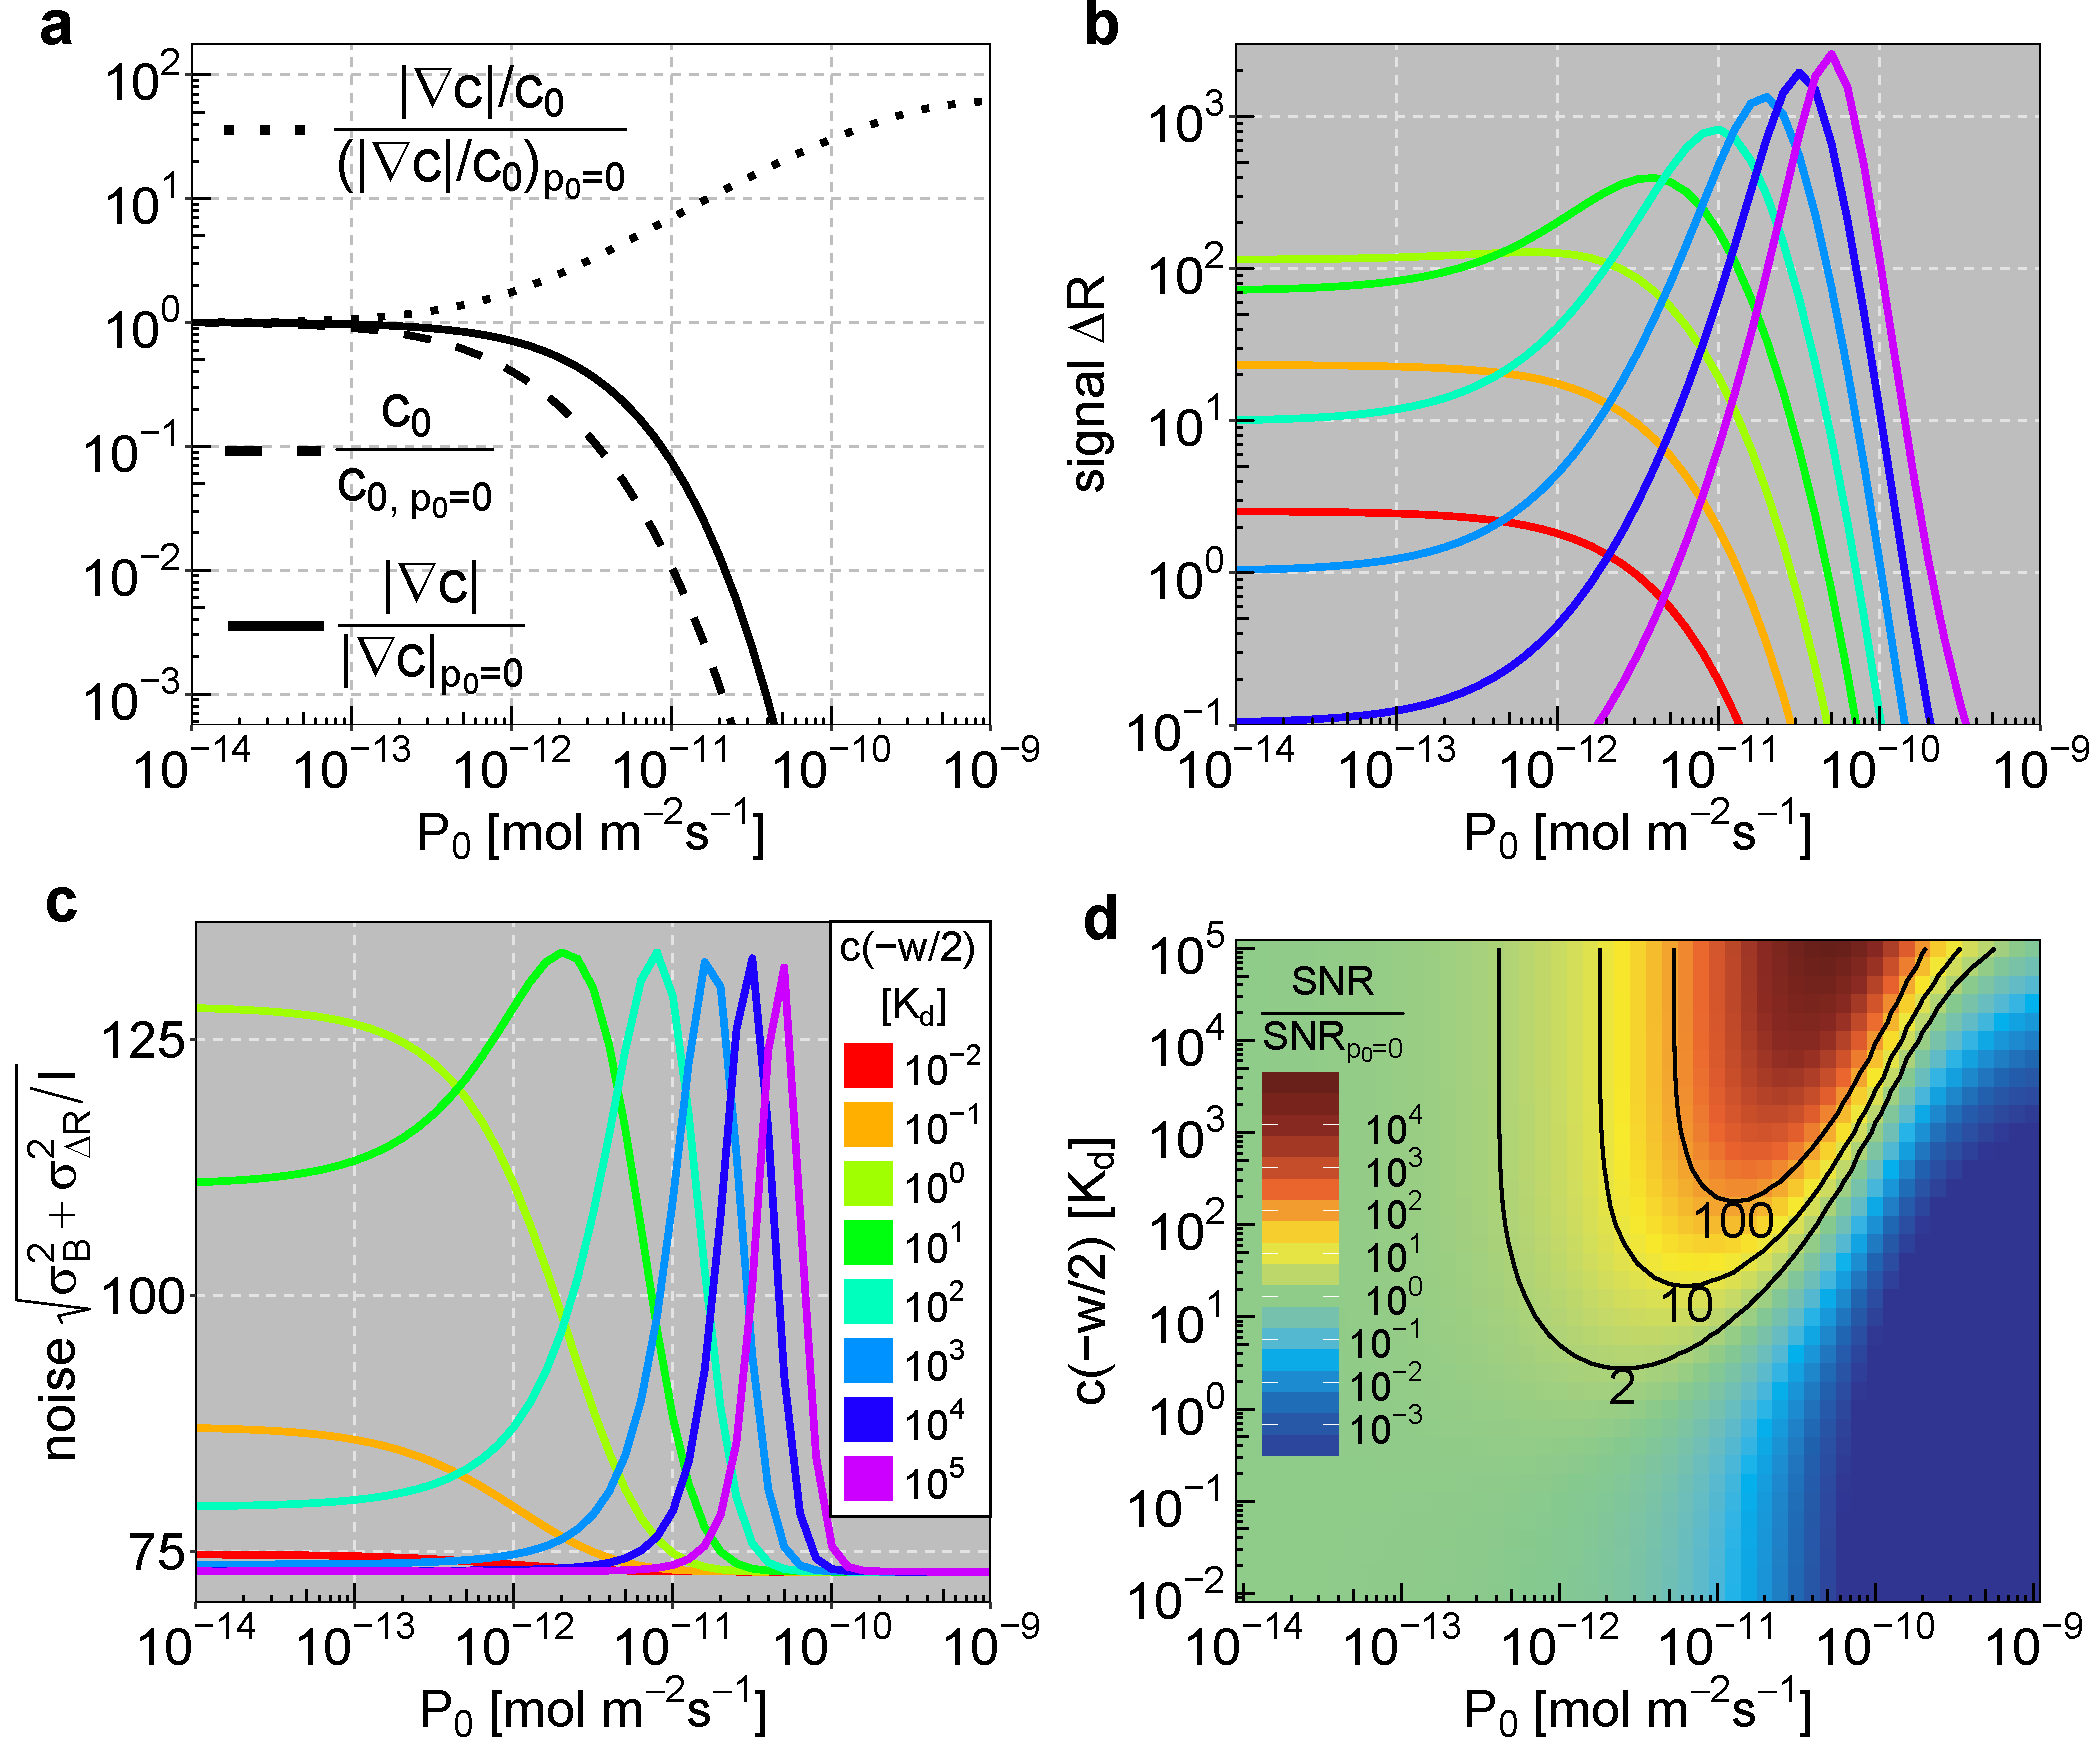
\includegraphics[scale=0.245]{../figures/fig3_pde_flux_plots}
	\caption{
		\linespread{1.0}
		Signal and noise analysis of the Fixed PDE secretion flux model.
		\textbf{a}. Mean cAMP concentration $c_0$ and gradient $|\vec{\nabla}c|$ across the cell surface, as a function of PDE secretion flux $P_0$. 
		\textbf{b}. Signal $\Delta R(P_0) \propto |\vec{\nabla}c|/(c_0 + K_d)^2$. Color legend is the same as in c.
		\textbf{c}. Noise $\sqrt{\sigma_B^2 + \sigma_{\Delta R}^2/I}$, with lower limit $\sigma_B = 73$ and upper limit $\sqrt{\sigma_B^2 + N/(4I)} \approx 134$. 
		\textbf{d}. Ratio of SNR and SNR with $P_0 = 0$. Most of the SNR enhancement results from the enhancement of the signal $\Delta R$. 
	}
	\label{fig:pde_flux_signal_noise}
\end{figure}

Finally, we consider the case of cAMP emitted by the point source in full 3D space. Without PDE, the solution of the steady-state diffusion equation for cAMP concentration $c(\vec{r})$ is equivalent to the electrostatic potential from the point charge located at origin, $c(\vec{r}) \sim 1/r$. With uniform PDE, the cAMP concentration becomes $c(r) = C_0 e^{-r/L}/r$ (SI, Section 8.3) and is equivalent to ion screening in classical plasma \cite{screening}, with $L$ having the role of Debye length. We again observe same effect on SNR at distances below $\sim 0.5\,\mathrm{mm}$ from the source (Fig.\ref{fig:pde_uniform_analytical}c,d, SI Fig.8).

%
%  Figure 4. Fixed PDE concentration models; microfluidic + spherical.
%
\begin{figure}
	\centering
	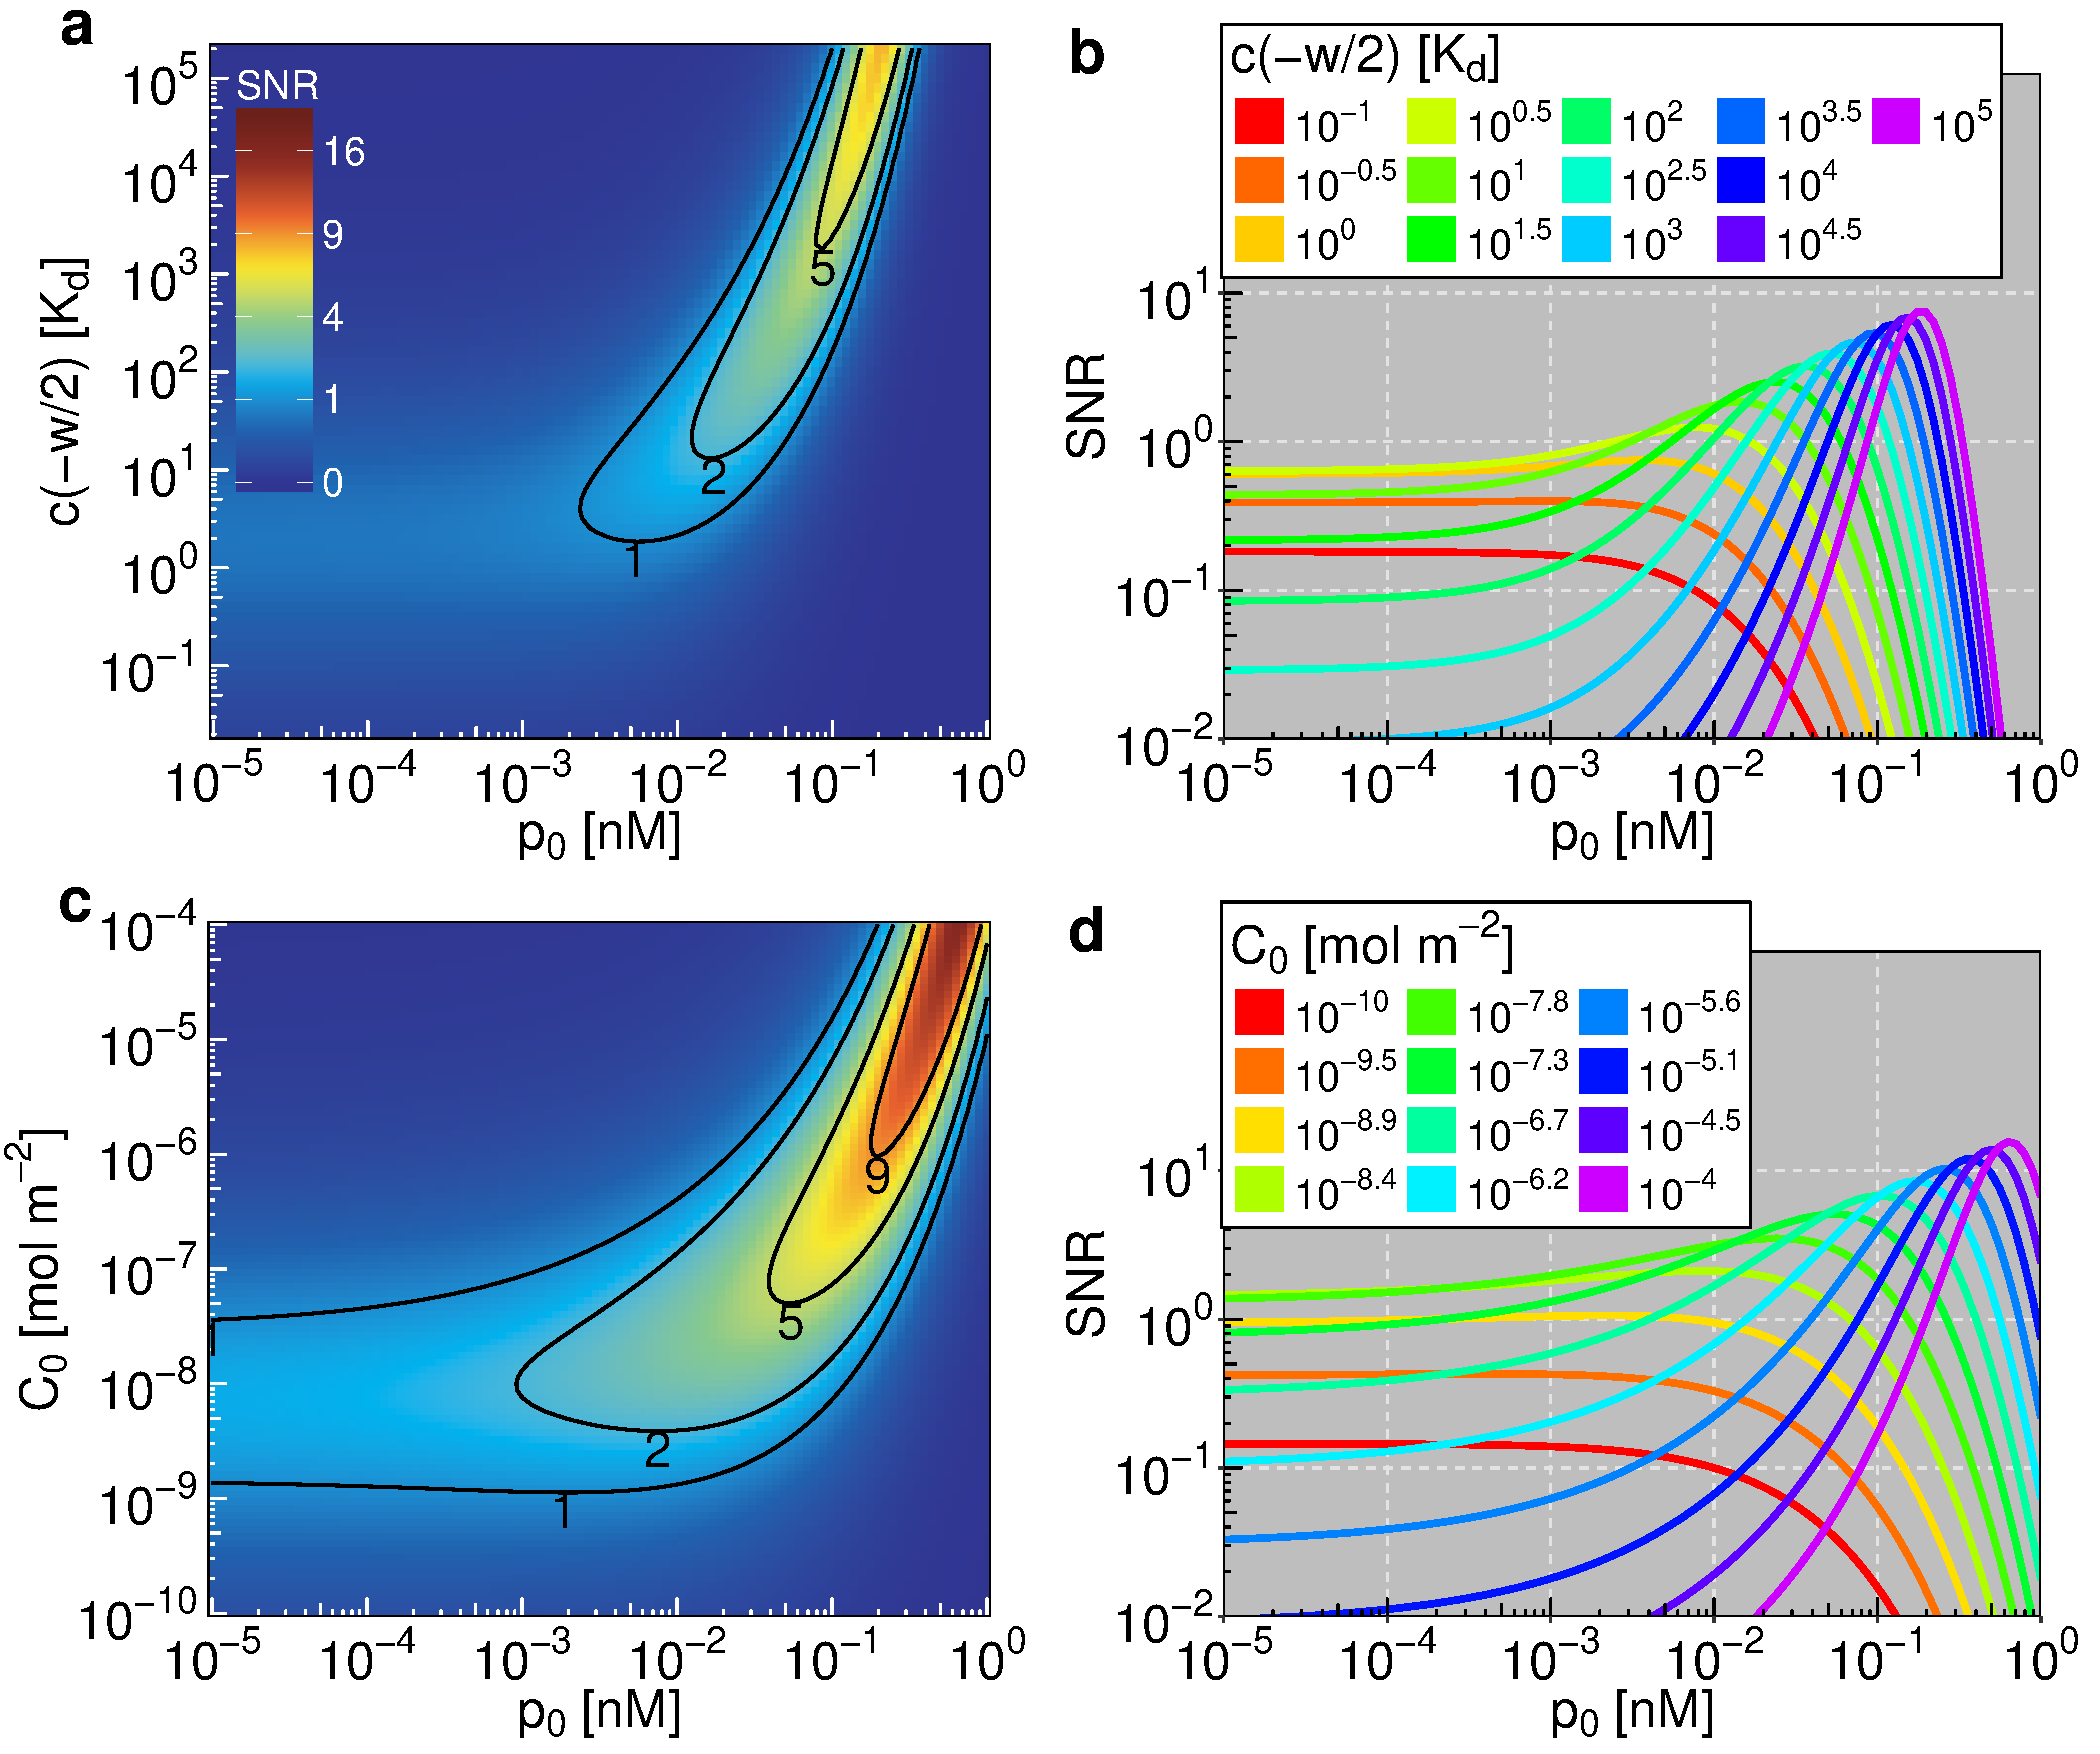
\includegraphics[scale=0.245]{../figures/fig4_analytical_pde_uniform_snr}
	\caption{
		\linespread{1.0}
		Analytical exact solutions for SNR for Fixed PDE concentration models.
		\textbf{a,b}. Microfluidic geometry: SNR as a function of PDE concentration $p_0$ and cAMP concentration on the left boundary $c(-w/2)$.
		\textbf{c,d}. cAMP point source $C_0 \delta(r)$ located at $\vec{r} = 0$: SNR as a function of cAMP source strength $C_0$ and $p_0$ at a distance $r = 225\,\mathrm{\mu m}$ from the source.
	}
	\label{fig:pde_uniform_analytical}
\end{figure}


%
% 	Conclusion / discussion
%
\emph{Concluding remarks.}--- In summary, we investigated the effects of extracellular PDE on cAMP gradient sensing in \emph{D. discoideum}. We find that PDE secretion by cells shifts their response towards higher cAMP concentrations (as expected) but can also greatly increase the SNR and broaden the range of signal detection. This contrasts an earlier conclusion reached using dimensional analysis \cite{mechanism1}. The SNR increase is directly related to the increase in the signal (differential receptor occupancy), while the noise has a PDE-independent upper bound. 

Our model results qualitatively agree with (i) previous observations of \emph{pdsA-} cells responding to a narrower range of cAMP concentrations \cite{pdsA1} and (ii) decrease in CI if the cells are starved for longer time periods, and exposed to the same gradient (Fig.4 in \cite{fisherStatic}) since the peak response would shift towards higher cAMP concentrations if the PDE accumulates in the environment. CI could also measured for the range of cAMP concentrations for both wild-type and \emph{pdsA-} cells and compared to the predictions of our model.

% Furthermore, the CI is observed to decrease if the cells are starved for longer time periods, and exposed to the same gradient $|\vec{\nabla} c| \approx 0.03 \,\mathrm{nM\,\mu m^{-1}}$, $c_0 \approx 30\,\mathrm{nM}$ (Fig.4 in \cite{fisherStatic}). This can also be explained by our model, since the peak of shifts towards higher cAMP concentrations if the PDE accumulates in the environment.

The effects discussed here also lead to different predictions between the experiments with static non-flowing gradients where cAMP gradients are affected by secreted PDE \cite{me,varnumsollStatic,fisherStatic}
and the experiments with static gradients establish with flow \cite{song,fuller-1,eberhard1}. The flow gradient experiments are considered advantageous since the cells are prevented to communicate with each other with cAMP (while not significantly distorting the local gradient around the cell \cite{ebFlow}), however they also completely wash away extracellular PDE (SI, Section 9).

Finally, we neglected the effects of PDE inhibitor, which is expected to get secreted under high PDE levels \cite{PdePdiKd} and would effectively increase the Michaelis-Menten constant of the cAMP-PDE interaction $K_M$ towards millimolar range \cite{KmcAMPPDEandPDI}.


\section*{Acknowledgments}

We thank Cornell ACCEL computer lab for the access to COMSOL Multiphysics
and MATLAB software, and anonymous referees for insightful suggestions.

\bibliography{references}%  Produces the bibliography via BibTeX.

\end{document}
